\documentclass{article}
\setlength{\parindent}{0pt}
\setlength{\parskip}{1em}
\setlength{\columnsep}{3cm}

\usepackage{xcolor}
\usepackage{multicol}
\usepackage{unicode-math}
\usepackage{listings}
\usepackage{lualatex-math}
\setmainfont[
  BoldFont={STIXTwoText-Bold},
  ItalicFont={STIXTwoText-Italic},
  BoldItalicFont={STIXTwoText-BoldItalic}
]{STIXTwoText-Regular}
\setmathfont{STIXTwoMath-Regular}

\usepackage{biblatex}
\addbibresource{references.bib}

\usepackage{tikz}
\usetikzlibrary{automata, trees, positioning, arrows, fit, matrix, shapes.geometric, shapes.misc, calc}
\pgfdeclarelayer{background}
\pgfdeclarelayer{foreground}
\pgfsetlayers{background,main,foreground}

\newcommand\Var[1]{\textcolor{blue}{#1}}
\newcommand\Num[1]{\textcolor{orange}{#1}}
\newcommand\Keyword[1]{{\textbf{\texttt{#1}}}}
\newcommand\Fun[1]{{\texttt{#1}}}

\lstnewenvironment{CITY}[1][]
{   
    \lstset{
        mathescape=true,
        basicstyle=\footnotesize, 
        basicstyle=\ttfamily,
        stringstyle=\color{teal},
        morestring=[b]",
        showstringspaces=false,
        keywords={,let,if,else,in,city,road,building,for,foreach,to,procedure,lambda,park,field,tree,junction,river,lake,restaurant, nil,},
        escapeinside={@}{@},
        xleftmargin=.04\textwidth,
        #1
    }
}
{}

\title{City}

\begin{document}

Cilj projektne naloge je izdelava domensko specifičnega jezika za opis infrastrukture v mestu.
Jezik morate zasnovati sami, torej sami določite sintakso in elemente jezika.
Jezik opisan v tem dokumentu naj služi predvsem za inspiracijo.

\section{Osnova}
Zahtevano je, da lahko z uporabo vašega jezika opišete vsaj zgradbe in ceste v mestu.
Na primer, z uporabo našega jezika lahko majhen izsek mesta opišemo takole \footnote{Primer je deloma izmišljen, čeprav opisane ceste in zgradbe res obstajajo v Fiesi, postavitev ni realna.}:

\begin{multicols}{2}
\begin{CITY}
  city "Fiesa" {
    road "Oljcna pot" {
      bend((@\Num{1}@, @\Num{1}@), (@\Num{2}@, @\Num{2}@), @\Num{20}@);
      bend((@\Num{2}@, @\Num{2}@), (@\Num{3}@, @\Num{1}@), @\Num{40}@);
      line((@\Num{2}@, @\Num{2}@), (@\Num{2}@, @\Num{5}@));
      bend((@\Num{2}@, @\Num{3}@), (@\Num{5}@, @\Num{4}@), @\Num{20}@);
      line((@\Num{5}@, @\Num{4}@), (@\Num{6}@, @\Num{4}@))
    };
    building "Soncne terase" {
      box((@\Num{3}@, @\Num{2}@), (@\Num{5}@, @\Num{3}@))
    };
    building "Dom Fiesa" {
      box((@\Num{0.5}@, @\Num{3.5}@), (@\Num{1.5}@, @\Num{2.5}@))
    };
    building "LaRocca" {
      box((@\Num{0.5}@, @\Num{5}@), (@\Num{1.5}@, @\Num{4}@))
    };
    building "Hotel Fiesa" {
      box((@\Num{1.75}@, @\Num{1.5}@), (@\Num{2.25}@, @\Num{1}@))
    }
  }
\end{CITY}

\columnbreak

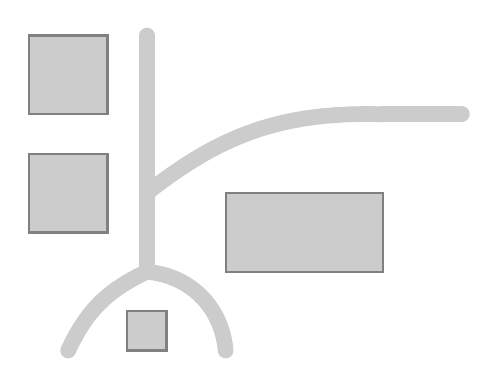
\begin{tikzpicture}
  \draw [line width=2mm, color=white!60!gray, line cap=round] (1, 1) to[bend left=20] (2, 2);
  \draw [line width=2mm, color=white!60!gray, line cap=round]  (2, 2) to[bend left=40] (3, 1);
  \draw [line width=2mm, color=white!60!gray, line cap=round]  (2, 2) to (2, 5);
  \draw [line width=2mm, color=white!60!gray, line cap=round]  (2, 3) to[bend left=20] (5, 4);
  \draw [line width=2mm, color=white!60!gray, line cap=round]  (5, 4) to (6, 4);

  \fill [thick, fill=white!60!gray, draw=gray] (3, 2) rectangle (5, 3);
  \fill [thick, fill=white!60!gray, draw=gray] (0.5, 3.5) rectangle (1.5, 2.5);
  \fill [thick, fill=white!60!gray, draw=gray] (0.5, 5) rectangle (1.5, 4);
  \fill [thick, fill=white!60!gray, draw=gray] (1.75, 1.5) rectangle (2.25, 1);

\end{tikzpicture}
\end{multicols}


\subsection{Konstrukti}
Vaš jezik mora vsebovati vsaj naslednje (ali ekvivalentne) konstrukte:

\subsubsection{Enota}
Enota služi kot nevtralen element (NO-OP).
\begin{CITY}
  nil
\end{CITY}

\subsubsection{Števila}
\begin{CITY}
  @\Num{1}@
  @\Num{1.2}@
\end{CITY}

\subsubsection{Nizi}
\begin{CITY}
  "NIZ"
\end{CITY}

\subsubsection{Točke}
S točkami lahko predstavimo lokacije na zemljevidu, v tem primeru je prva komponenta longituda, druga komponenta pa je latituda.
\begin{CITY}
  (@\Var{X}@, @\Var{Y}@)
\end{CITY}

\subsubsection{Bloki}
Blok \Keyword{city} predstavlja mesto, ki ga opisujemo.
Vsebuje lahko bloke za opis cest in zgradb.
To je glaven element v jeziku.
\begin{CITY}
  city "NAME" {
    @\Var{BLOCKS}@
  }
\end{CITY}

Blok \Keyword{road} predstavlja cesto.
Vsebuje lahko ukaze za izris, ki izrišejo črte.
\begin{CITY}
  road "NAME" {
    @\Var{COMMANDS}@
  }
\end{CITY}

Blok \Keyword{builing} predstavlja zgradbo.
Vsebuje lahko ukaze za izris, ki izrišejo obrobo zapolnjenega lika.
Obroba lika mora biti zaključena, torej končna lokacija mora biti enaka prvi.
\begin{CITY}
  building "NAME" {
    @\Var{COMMANDS}@
  }
\end{CITY}

\subsubsection{Ukazi}

Bloka \Keyword{road} in \Keyword{building} lahko vsebujeta naslednje ukaze za izris.

Ukaz \Fun{line} izriše črto, med podanima lokacijama.
\begin{CITY}
  line(@\Var{POINT}@, @\Var{POINT}@)
\end{CITY}

Ukaz \Fun{bend} izriše krivuljo, med podanima lokacijama.
Podani kot določa stopnjo ukrivljenosti.
Če je kot $0^\circ$ se izriše ravna črta, če je kot $45^\circ$ se izriše približek četrtine krožnice.
Pozitivni koti pomenijo, da je krivulja nagnjena v levo, negativni koti pa pomenijo, da je krivulja nagnjena v desno.

\begin{CITY}
  bend(@\Var{POINT}@, @\Var{POINT}@, @\Var{ANGLE}@)
\end{CITY}

Ukaz \Fun{box} izriše pravokotnik, med podanima lokacijama.
Torej prva lokacija je zgornji levi kot pravokotnika, druga lokacija pa je spodnji desni kot.
\begin{CITY}
  box(@\Var{POINT}@, @\Var{POINT}@)
\end{CITY}

Ukaz \Fun{circ} izriše krog z izbranim polmerom na podani lokaciji.
Ta lokacija predstavlja center kroga.
\begin{CITY}
  circ(@\Var{POINT}@, @\Var{RADIUS}@)
\end{CITY}

\section{Nadgradnja}
Jezik razširite še s katerim od naslednjih konstruktov (oz. dodajte poljubne konstrukte po lastnem okusu):

\subsection{Spremenljivke}
Konstrukt \Keyword{let} omogoča, da ustvarite novo konstanto.
Tako boste lahko določene točke shranili in jih nato večkrat uporabili.
Predlagamo, da uporabite dinamično in strogo tipiziranje.
Po želji lahko dodate tudi spremenljivke.

\begin{CITY}
  road "Oljcna pot" {
    let p = (@\Num{2}@, @\Num{2}@);
    let q = (@\Num{5}@, @\Num{4}@);

    bend((@\Num{1}@, @\Num{1}@), p, @\Num{20}@);
    bend(p, (@\Num{3}@, @\Num{1}@), @\Num{40}@);
    line(p, (@\Num{2}@, @\Num{5}@));
    bend((@\Num{2}@, @\Num{3}@), q, @\Num{20}@);
    line(q, (@\Num{6}@, @\Num{4}@))
  }
\end{CITY}

\subsection{Izjave}
Pogosto je koristno, da lahko izračunamo novo lokacijo na podlagi parametrov ali obstoječih lokacij.
Da boste lahko dobili elemente točk je potrebno vgraditi funkciji \Fun{fst} in \Fun{snd}, ki vrneta prvi in drugi element točke.

\begin{CITY}
  road "Oljcna pot" {
    let bound = @\Num{1}@;
    let s = (bound, bound);
    let p = (fst(s) + @\Num{1}@, snd(s) + @\Num{1}@);
    let q = (@\Num{5}@, @\Num{4}@);

    bend(s, p, @\Num{20}@);
    bend(p, (@\Num{3}@, @bound@), @\Num{40}@);
    line(p, (@\Num{2}@, @\Num{5}@));
    bend((@\Num{2}@, @\Num{3}@), q, @\Num{20}@);
    line(q, (@\Num{6}@, @\Num{4}@))
  }
\end{CITY}

\subsection{Kontrola toka}
Ponavljajoče elemente lahko lažje izrišemo, če imamo na voljo zanko \Keyword{for}.
Tako lahko na primer izrišemo vrstne hiše.
Lahko pa izrišemo tudi bolj kompleksne oblike, ki nam bodo prišle prav pri testiranju.
Včasih je uporabno (še posebej znotraj zanke), da lahko izrišemo nekatere elemente pogojno.
Za to lahko uporabimo vejitev \Keyword{if}.
Za podporo vejitev je potrebno dodati še Boolove vrednosti \Keyword{true} in \Keyword{false}, Boolove operatorje in operatorje za primerjavo.

\begin{CITY}
  building "Hotel Fiesa" {
    if n > @\Num{1}@ {
      line((@\Num{1}@, @\Num{1}@), (@\Num{2}@, @\Num{2}@))
    } else {
      line((@\Num{2}@, @\Num{1}@), (@\Num{1}@, @\Num{2}@))
    }

    for i = @\Num{1}@ to @\Num{3}@ {
      box((@\Num{1}@, i), (@\Num{2}@, i + @\Num{1}@))
    }
  }
\end{CITY}

\subsection{Abstrakcija}
Določene kompleksne elemente lahko ponovimo na poljubnih mestih, tako da dodamo procedure \Keyword{procedure} in funkcije \Keyword{lambda}.
Poleg tega, pa lahko uporabimo ta konstrukta za poljubne izračune, kar še dodatno dvigne izraznost jezika.
Za rekurzivne funkcije lahko dodamo konstrukt $\Keyword{rec let}$.
Če so spremenljivke dinamično tipizirane pa lahko rekurzijo podpremo tudi brez dodatnih konstruktov, tako da definiramo operator, ki nam vrne fiksno točko \Fun{fix} \footnote{https://en.wikipedia.org/wiki/Fixed-point\_combinator}.
Predstavljene procedure in funkcije vrnejo zadnjo vrednost, lahko pa definiramo tudi ukaz \Keyword{return}, ki ga lahko uporabimo tudi za predčasen zaključek izvajanja.

\begin{CITY}
  procedure row(p) {
    for i = @\Num{1}@ to @\Num{3}@ {
      box((fst(p), snd(p) + i), (fst(p) + @\Num{1}@, snd(p) + i + @\Num{1}@))
    }
  };

  building "Hotel Fiesa" {
    let square = lambda(x) {x * x};
    row((@\Num{1}@, square(@\Num{2}@)))
  }
\end{CITY}

\subsection{Seznami}
Točke lahko služijo tudi kot pari.
Z uporabo parov je mogoče enostavno podpreti enojno povezane sezname.
Za rep para lahko uporabimo enoto \Keyword{nil}.
Podpremo lahko tudi zanko \Keyword{foreach}, ki se izvede za vsak element seznama.
Prav tako pa lahko definiramo tudi lepšo sintakso, ki se pretvori v predstavitev s pari.

\begin{CITY}
  building "Hotel Fiesa" {
    let list = (@\Num{1}@, (@\Num{2}@, (@\Num{3}@, nil)));

    foreach x in list {
      box((@\Num{1}@, x), (@\Num{2}@, x + @\Num{1}@))
    };

    let fancy = [@\Num{1}@, @\Num{2}@, @\Num{3}@]
  }
\end{CITY}


\subsection{Sintaktični sladkor}
Poleg (ali namesto) ukazov lahko uporabimo tudi bolj strnjeno in elegantno sintakso.
Tukaj namesto ukaza \Fun{line} uporabljamo operator, prav tako pa združimo dele ceste, ki se držijo skupaj (tako se lahko izognemo podvajanju točk).
Sintaktični sladkor lahko dodate kjerkoli se vam zdi smiselno, tako bo vaš jezik bolj prijeten za uporabo.

\begin{CITY}
  road "Oljcna pot" {
    (@\Num{1}@, @\Num{1}@) -- bend @\Num{20}@ (@\Num{2}@, @\Num{2}@) -- bend @\Num{40}@ (@\Num{3}@, @\Num{1}@);
    (@\Num{2}@, @\Num{2}@) -- (@\Num{2}@, @\Num{5}@);
    (@\Num{2}@, @\Num{3}@) -- bend @\Num{20}@ (@\Num{5}@, @\Num{4}@) -- (@\Num{6}@, @\Num{4}@);
  }
\end{CITY}

\subsection{Dodatni ukazi}
Poleg osnovnih ukazov za izris lahko dodamo še druge: ukaz za izris elipse, dele krožnic, črte in krivulje sestavljene iz več segmentov (to je eden od načinov da se izognemo podvajanju točk), lahko definiramo razširjen ukaz \Fun{bend}, kjer se kota na vsaki strani razlikujeta, dodamo lahko parameter, ki nam pove kako ohlapna naj bo krivulja, lahko pa dodamo tudi ukaz \Fun{curve}, ki nam omogoča da prosto izberemo kontrolne točke Bezierjeve krivulje.
Poleg teh pa lahko dodate tudi poljubne ukaze po vašem okusu.

\begin{CITY}
  ellip(@\Var{POINT}@, @\Var{AXIS}@, @\Var{AXIS}@)

  arc(@\Var{POINT}@, @\Var{ANGLE}@, @\Var{ANGLE}@)

  polyline(@\Var{POINTS}@)

  polyspline(@\Var{POINTS}@)

  bend(@\Var{POINT}@, @\Var{POINT}@, @\Var{ANGLE}@, @\Var{ANGLE}@)

  bend(@\Var{POINT}@, @\Var{POINT}@, @\Var{ANGLE}@, @\Var{ANGLE}@, @\Var{LOOSENESS}@)

  curve(@\Var{POINT}@, @\Var{POINT}@, @\Var{CONTROL}@)

  curve(@\Var{POINT}@, @\Var{POINT}@, @\Var{CONTROL}@, @\Var{CONTROL}@)
\end{CITY}

\subsection{Dodatni elementi}
Na zemljevid lahko dodamo še ostale elemente mest, kot so reke, jezera, parke, polja.
Mesta pa lahko vsebujejo tudi točkovne elemente, kot so drevesa, križišča, restavracije.
Poleg teh pa lahko dodate tudi poljubne elemente po vašem okusu.

\begin{CITY}
  river "NAME" {
    @\Var{COMMANDS}@
  }

  lake "NAME" {
    @\Var{COMMANDS}@
  }

  park "NAME" {
    @\Var{COMMANDS}@
  }

  field {
    @\Var{COMMANDS}@
  }

  tree @\Var{POINT}@

  junction @\Var{POINT}@

  restaurant "NAME" @\Var{POINT}@
\end{CITY}
\end{document}
